\documentclass {article}
\usepackage [magyar]{babel}
\usepackage { t1enc }
\usepackage[inline]{enumitem}
\usepackage{lipsum}
\usepackage{xcolor}
\usepackage{graphicx}
\usepackage{hulipsum}
\usepackage{float}
\usepackage{subcaption}
\usepackage{wrapfig}




\begin {document}
\listoffigures




\begin{itemize*}[afterlabel=~,%
itemjoin=\hspace{1em},%
itemjoin*={\hspace{1em}és }]
\item[*] elso elem
\item[*] masodik elem
\item[*] harmadik elem

\end{itemize*}

\begin{enumerate}
\item egy
\begin{enumerate}
\item második szint!
\begin{enumerate}
\item harmadik szint!
\begin{enumerate}
\item negyedik szint!
\end{enumerate}
\end{enumerate}
\end{enumerate}
\item ketto
\end{enumerate}

\lipsum[1]

\begin{enumerate}[resume]
\item\label  három

\item[*]\label  négy
\stepcounter{enumi}
\item öt
\end{enumerate}

\begin{description}[align=parleft,%
leftmargin=*,widest={hosszabb}, font=\slshape, style=nextline]
\item \hulipsum[2]
\item[címke] \hulipsum[1]
\item[ez egy hosszabb címke!] \hulipsum[3]
\end{description}

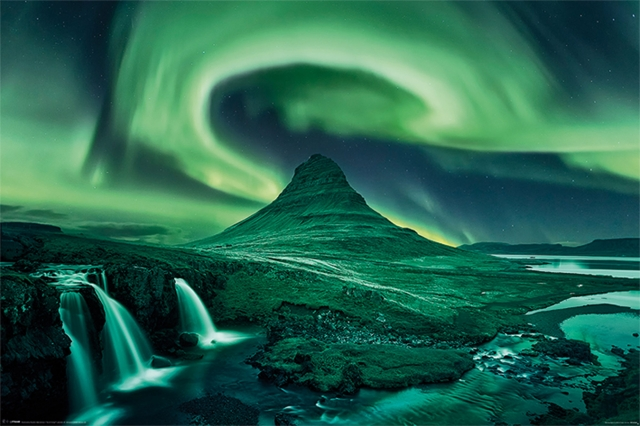
\includegraphics[width=5cm, height=5cm]{../forras/110.jpg}

\begin{figure}[b]
\hulipsum[1]
\centering

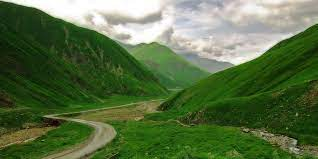
\includegraphics[width=5cm, height=5cm]{../forras/111.jpg}
\caption[ábra]{Szép zöld táj}
\ref{} 	
	\begin{subfigure}{5cm}
 	\subref{}
	\centering
	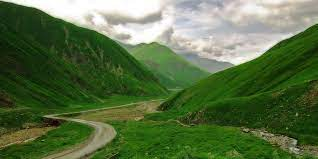
\includegraphics[width=5cm, height=5cm, angle=180]{../forras/111.jpg}
	\caption[részábra]{Szép zöld táj}
	\end{subfigure}

\hulipsum[1]
\end{figure}









\vspace{10cm}






\begin{tabular}{c || ccc|}
  & egy & kettő & három \\ 
\cline{1-4}
Helló világ! & négy & öt & hat \\
\cline{2-4}  
  & hét & nyolc & kilenc \\
\cline{2-2}\cline{4-4}
Lórum ipse & tíz & & tizenkettő \\
\cline{1-4}

\end{tabular}


\end {document}